\chapter*{Introduction}
\markright{Introduction}
\label{intro}
\phantomsection
\addcontentsline{toc}{chapter}{Introduction}

In the last few years the stereoscopic technique has become a great part of the image and video processing.\\
In medical diagnosis and endoscopic surgery, fault detection in manufactory industry, army and arts
multiview imaging is considered as a key enabler  for professional added value services.\\
\begin{figure}[h!]
\centering
\begin{subfigure}[]{0.5\textwidth}
		\centering
        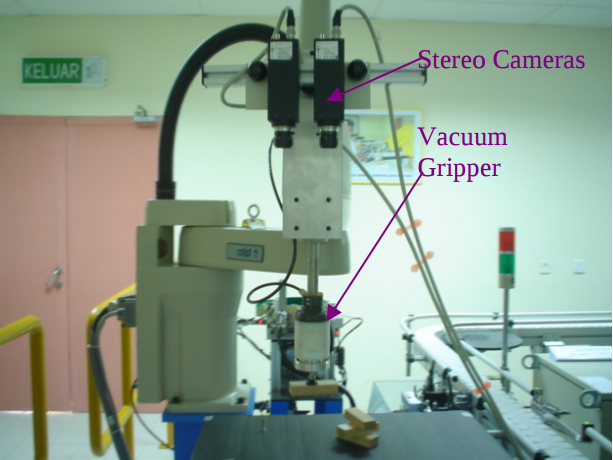
\includegraphics[width=0.7\textwidth]{./img/bin_pick.png}
                \caption{\scriptsize{In bin picking applications stereo vision helps to reconstruct the 3D environment and detect the part of the object to be robotically picked}}
\end{subfigure}% 
~ \quad
\begin{subfigure}[]{0.5\textwidth}
	\centering
	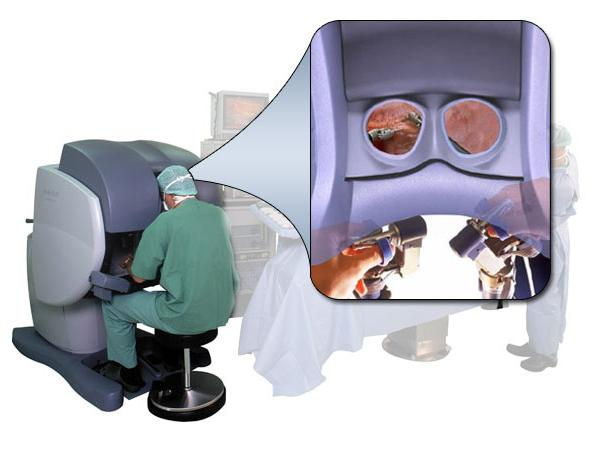
\includegraphics[width=0.7\textwidth]{./img/da_vinci.jpg}
          \caption{\scriptsize{Surgical robot \textit{Da vinci} is provided with a stereoscopic camera that allows a tridimensional view of the operative filed.}}
\end{subfigure} 
\caption{\small{Stereoscopy in medical and industrial field}}
\end{figure}

Nowdays stereoscopic techniques are also used in people tracking and mobile robotics
navigation for economic reasons and to improve performances.\\
\begin{figure}[h!]
\centering
\begin{subfigure}[]{0.5\textwidth}
		\centering
        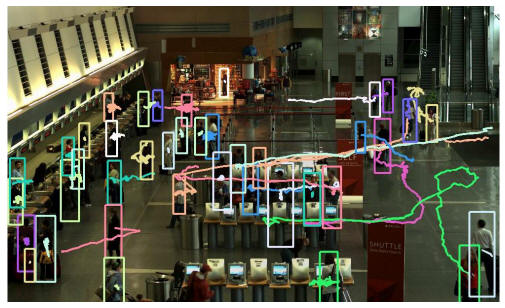
\includegraphics[width=0.7\textwidth]{./img/tracking.jpg}
                \caption{\scriptsize{In people tracking application stereo vision improves segmentation thanks to depth information and it's less sensible to light changes.}}
\end{subfigure}% 
~ \quad
\begin{subfigure}[]{0.5\textwidth}
		\centering
        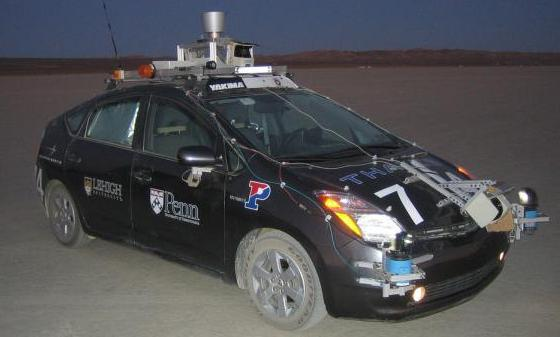
\includegraphics[width=0.7\textwidth]{./img/little_ben.jpg}
                \caption{\scriptsize{In mobile robotics navigation stereo vision has became the first choice technology because it provids a lot of quality data for low costs.}}
\end{subfigure} 
\caption{\small{Stereoscopy application's fields}}
\end{figure}
Finally the worldwide success of movie releases and  3D video games and the deployment of 3D televisions made the nonprofessional user aware about a new type of multimedia entertainment experience.\\

\begin{figure}[h!]
\centering
\begin{subfigure}[]{0.4\textwidth}
		\centering
        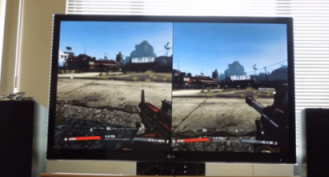
\includegraphics[width=0.7\textwidth]{./img/games1.png}
                \caption{\scriptsize{Stereo video frames, left and right.\newline}}
\end{subfigure}
\begin{subfigure}[]{0.4\textwidth}
		\centering
        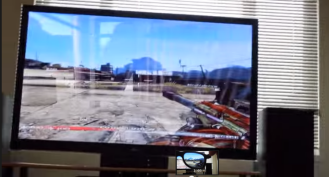
\includegraphics[width=0.7\textwidth]{./img/games2.png}
                \caption{\scriptsize{Overlap of the two frames.}}
\end{subfigure} 
\begin{subfigure}[]{0.4\textwidth}
		\centering
        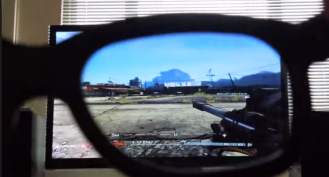
\includegraphics[width=0.7\textwidth]{./img/games3.png}
                \caption{\scriptsize{3D view with specific glasses}}
\end{subfigure}%
\begin{subfigure}[]{0.4\textwidth}
		\centering
        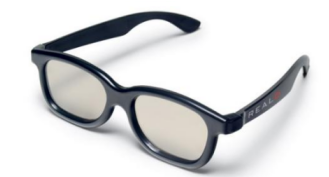
\includegraphics[width=0.7\textwidth]{./img/games4.png}
                \caption{\scriptsize{Polarized glasses for 3D view}}
\end{subfigure} 
\caption{\small{Stereoscopy in 3D video games}}
\end{figure}

The increase of production and distribution of these contents leads to the concerns over content copyright protection.\\
Digital watermarking can be considered as the most flexible property right protection technology, since it adds some information (a mark, i.e. copyright information) in the
original content without altering its visual quality so that such a marked content can be further distributed/consumed by another user without any restriction; still, the legitimate/illegitimate usage can be determined at any moment by detecting the mark. In same case the watermarking protection mechanism, instead of restricting the media copy/distribution/consumption, provides means for tracking the source of the content illegitimate usage.\\
The purpose of this thesis is to provide a new watermarking system for copyright protection of stereo videos. The method operates in the frequency and in the spatial domain, by embedding a pseudo-random sequence of real numbers in a selected set of DFT coefficients of the left image and then by spatially adding to the right image the reference watermark distorted according to the depth information prior to insertion.\\

